\documentclass[journal]{IEEEtran}
%\documentclass[12pt,journal,draftclsnofoot,onecolumn]{IEEEtran}
%\documentclass[conference]{IEEEtran}

\IEEEoverridecommandlockouts

\usepackage{etex}

%Fixing IEEEtran.cls bug with [english]{babel}
\makeatletter
\def\markboth#1#2{\def\leftmark{\@IEEEcompsoconly{\sffamily}\MakeUppercase{\protect#1}}%
\def\rightmark{\@IEEEcompsoconly{\sffamily}\MakeUppercase{\protect#2}}}
\makeatother

% \usepackage{t1enc}

%\usepackage[utf8x]{inputenc}
\usepackage[english]{babel}
\selectlanguage{english}
\usepackage{color}
\usepackage{lipsum}% http://ctan.org/pkg/lipsum
%\usepackage{caption}
\usepackage{cite}
\usepackage[pdftex]{graphicx}
%\usepackage{subfig}
%\usepackage{subcaption}
\usepackage{amsmath}
\usepackage{amsfonts}
\usepackage{array}
\usepackage{verbatim}
\usepackage{listings}
%\usepackage{algorithm}
%\usepackage{algorithmic}
%\usepackage{algpseudocode}
\usepackage{hyperref}
\usepackage{url}
\usepackage{enumerate}
\usepackage{multirow}

\usepackage{epsfig}
\usepackage{epstopdf}
\usepackage{multicol}% http://ctan.org/pkg/multicols
\usepackage[font=footnotesize]{caption}
\usepackage[font=scriptsize]{subcaption}
% Tikz
\usepackage{tikz}
\usepackage{pgfplots}
\pgfplotsset{compat=newest}
\pgfplotsset{plot coordinates/math parser=false}
\newlength\fheight
\newlength\fwidth
\usetikzlibrary{patterns,decorations.pathreplacing,backgrounds,calc}
\definecolor{SchoolColor}{RGB}{0.71, 0, 0.106}%181,0,27} unipd red
\definecolor{chaptergrey}{rgb}{0.61, 0, 0.09} % dialed back a little
\definecolor{midgrey}{rgb}{0.4, 0.4, 0.4}
\definecolor{chaptergreen}{rgb}{0.09, 0.612, 0}
\definecolor{chapterpurple}{rgb}{0.522, 0, 0.612}
\definecolor{chapterlightgreen}{rgb}{0, 0.612, 0.522}

%\raggedbottom

% Pseudocode
\usepackage{algorithm}
\usepackage[noend]{algpseudocode}
\renewcommand\algorithmicthen{}
\renewcommand\algorithmicdo{}
\usepackage{lscape}
\usepackage{setspace}

\addto\captionsenglish{\renewcommand{\figurename}{Fig.}}

\newcommand{\field}[1]{\mathbb{#1}}

\DeclareMathOperator*{\argmin}{arg\,min}
\DeclareMathOperator*{\argmax}{arg\,max}
\renewcommand{\arraystretch}{2}

\newcommand{\DP}[1]{\textbf{(DP: #1)}}
\newcommand{\el}[1]{\textr{(EL says: #1)}}
\newcommand{\fm}[1]{\texbf{(FM says: #1)}}

\usepackage{threeparttable}
%\usepackage[table,xcdraw]{xcolor}
\usepackage{tabularx}
   \usepackage{multirow}
   \usepackage{booktabs}
\newcommand{\tabitem}{~~\llap{\textbullet}~~}
   \usepackage{array, blindtext}
   \usepackage{wrapfig}
\usepackage{pdfpages}
\usepackage[acronym]{glossaries}

% use tikArchiviz images or eps
\newif\iftikz
\tikztrue

\graphicspath{{./figures/}}

\title{Heuristic optimization of Distributed Storage Network techniques}
\author{\IEEEauthorblockN{Federico Mason$^*$, Davide Peron$^*$, Enrico Lovisotto$^*$}\\
\small{{$^*$Department of Information Engineering, University of Padova -- Via Gradenigo, 6/b, 35131 Padova, Italy\\
Email: {\tt\{masonfed,perondav,lovisott\}@dei.unipd.it}\\}}
}

% Reduce the space below figs.
%\setlength{\belowcaptionskip}{-0.7cm}

%% Glossary
\newacronym{dsn}{DSN}{Distributed Storage Network}
\newacronym{edfc}{EDFC}{Exact Decentralized Fountain Codes}
\newacronym{adfc}{ADFC}{Approximate Decentralized Fountain Codes}
\newacronym{sa}{SA}{Simulated Annealing}
\newacronym{ga}{GA}{Genetic Algorithm}
\newacronym{jb}{JB}{Jumping Ball}
\newacronym{wsn}{WSN}{Wireless Sensor Network}
\glsresetall
\begin{document}

\setlength{\belowcaptionskip}{-0.2cm}

% reduce space after title
\makeatletter
\patchcmd{\@maketitle}
  {\addvspace{0.5\baselineskip}\egroup}
  {\addvspace{-1.2\baselineskip}\egroup}
  {}
  {}
\makeatother

\maketitle

\begin{abstract}
In some previous works about \gls{dsn}, two packet spreading algorithm are presented, \gls{edfc} and \gls{adfc}.

Unfortunately the tuning of their fundamental parameters, $x_d$ and $\nu(d)$ respectively, was not thoroughly investigated.

We try to perform such tuning applying some heuristic optimization techniques, such as \emph{Simulated Annealing} and \emph{Genetic Algorithm}, in order to explore the solution space of the problem.

\end{abstract}

\begin{IEEEkeywords}
Distributed Storage Networks, sensors, heuristic optimization
\end{IEEEkeywords}

\glsresetall
\label{sec:introduction}
We consider a \gls{wsn} whose nodes are distributed over a known region.
Some of them, called \textit{sensing nodes}, collect and deploy data from the environment (temperature, pressure, motion data, \ldots) while the others, called \textit{caching nodes}, simply store data coming from \textit{sensing nodes}.

In literature, a \gls{wsn} often has a central node, a powered sink connected to the internet.
Such special node receives all information collected by the nodes in the network and provides it to the users.

However, in our paper, following what has been done in \cite{Lin2007}, we get rid of this assumption.
Users then must collect the data stored in the network visiting the geographical region in which system is located.

In such a scenario, a randomly picked number of the nodes is visited by a user.
Our reference paper \cite{Lin2007}, guarantees source packets decodability using \emph{Random Fountain Codes}, combining and spreading $K$ source packets across $N$ total nodes such that, using any group of $K+\epsilon$ of them (with $\epsilon$ constant), the original information can be successfully retrieved with high probability.

The challenge here is to keep the communication cost at a minimum level, while keeping the failure probability low.

Traditional but expensive two-way packet delivery is then discarded, in favour of one-way \emph{random walks}, where only neighbours knowledge is required locally.
Random walks are designed according to \emph{Metropolis algorithm} such that the number of packets reaching each node resembles the Robust Soliton distribution, whose optimal decoding properties are known\cite{Luby}.

In this paper, we are going to find the optimal $x_d$ parameter for \gls{edfc} with three heuristic tecniques.
The optimal configurations are then tested with a network simulator, and further analysis is performed.

The article is structured in three sections.

In \autoref{sec:tech_approach} we present in detail the heuristic algorithms employed, first with a general description of the framework and then fucusing on our specific problem.

In \autoref{sec:results} we present the results obtained using the optimal parameter configuration in the simulator we have implemented.

\section{Technical Approach}
\label{sec:tech_approach}

\section{Results}
\label{sec:results}
\begin{figure}
  \centering
    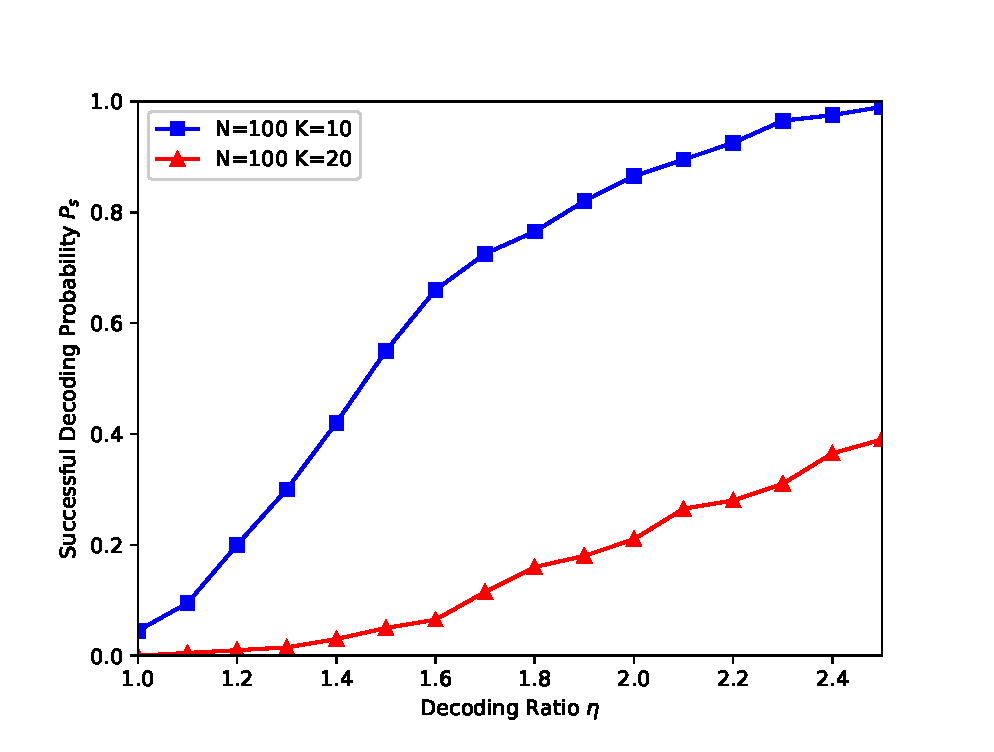
\includegraphics[width=0.9\columnwidth]{ratiovsprob.eps}
  \caption{Successfull decoding probability $P_s$ for different values of $N$, $K$ and decoding ratio $\nu$.}
  \label{fig:ratiovsprob}
\end{figure}

\section{Conclusions And Future Work}
\label{sec:conclusions}

\bibliographystyle{IEEEtran}
\bibliography{bibliography}

\end{document}
